\documentclass[10pt,letterpaper]{article}\usepackage[]{graphicx}\usepackage[]{color}
%% maxwidth is the original width if it is less than linewidth
%% otherwise use linewidth (to make sure the graphics do not exceed the margin)
\makeatletter
\def\maxwidth{ %
  \ifdim\Gin@nat@width>\linewidth
    \linewidth
  \else
    \Gin@nat@width
  \fi
}
\makeatother

\definecolor{fgcolor}{rgb}{0.345, 0.345, 0.345}
\newcommand{\hlnum}[1]{\textcolor[rgb]{0.686,0.059,0.569}{#1}}%
\newcommand{\hlstr}[1]{\textcolor[rgb]{0.192,0.494,0.8}{#1}}%
\newcommand{\hlcom}[1]{\textcolor[rgb]{0.678,0.584,0.686}{\textit{#1}}}%
\newcommand{\hlopt}[1]{\textcolor[rgb]{0,0,0}{#1}}%
\newcommand{\hlstd}[1]{\textcolor[rgb]{0.345,0.345,0.345}{#1}}%
\newcommand{\hlkwa}[1]{\textcolor[rgb]{0.161,0.373,0.58}{\textbf{#1}}}%
\newcommand{\hlkwb}[1]{\textcolor[rgb]{0.69,0.353,0.396}{#1}}%
\newcommand{\hlkwc}[1]{\textcolor[rgb]{0.333,0.667,0.333}{#1}}%
\newcommand{\hlkwd}[1]{\textcolor[rgb]{0.737,0.353,0.396}{\textbf{#1}}}%
\let\hlipl\hlkwb

\usepackage{framed}
\makeatletter
\newenvironment{kframe}{%
 \def\at@end@of@kframe{}%
 \ifinner\ifhmode%
  \def\at@end@of@kframe{\end{minipage}}%
  \begin{minipage}{\columnwidth}%
 \fi\fi%
 \def\FrameCommand##1{\hskip\@totalleftmargin \hskip-\fboxsep
 \colorbox{shadecolor}{##1}\hskip-\fboxsep
     % There is no \\@totalrightmargin, so:
     \hskip-\linewidth \hskip-\@totalleftmargin \hskip\columnwidth}%
 \MakeFramed {\advance\hsize-\width
   \@totalleftmargin\z@ \linewidth\hsize
   \@setminipage}}%
 {\par\unskip\endMakeFramed%
 \at@end@of@kframe}
\makeatother

\definecolor{shadecolor}{rgb}{.97, .97, .97}
\definecolor{messagecolor}{rgb}{0, 0, 0}
\definecolor{warningcolor}{rgb}{1, 0, 1}
\definecolor{errorcolor}{rgb}{1, 0, 0}
\newenvironment{knitrout}{}{} % an empty environment to be redefined in TeX

\usepackage{alltt}
\usepackage[top=0.8in, bottom=0.8in, left=0.8in, right=0.8in]{geometry}
\usepackage{amsmath}
\usepackage{graphicx}
\usepackage{hyperref}
\usepackage{setspace}
\usepackage{amssymb}
\usepackage{pdfpages}
\usepackage[table, dvipsnames]{xcolor}
\usepackage{caption,booktabs}
\usepackage[singlelinecheck=false ]{caption}
\usepackage{fancyvrb}
\usepackage{Sweave}
\usepackage[most,breakable]{tcolorbox}
\usepackage{environ}
\usepackage{array}
\usepackage[mathscr]{euscript}
\usepackage{fancybox}
\usepackage{shellesc}
\usepackage{xcolor,soul}
\tcbuselibrary{breakable}
\usepackage{animate}

%\renewcommand{\rmdefault}{bch} % change default font
\usepackage[english]{babel}
\usepackage[utf8]{inputenc}
\usepackage{tikz}
\usetikzlibrary{calc}
\usetikzlibrary{shapes}
\usepackage{enumitem}
\usepackage{bm}
\usetikzlibrary{arrows,decorations.pathmorphing,backgrounds,fit,positioning,shapes.symbols,chains}


\DefineVerbatimEnvironment{Sinput}{Verbatim}{xleftmargin=2em,frame=single}
\DefineVerbatimEnvironment{Soutput}{Verbatim}{xleftmargin=2em,frame=single}

%\captionsetup{
%	justification = centering
%}

\doublespacing
\IfFileExists{upquote.sty}{\usepackage{upquote}}{}
\begin{document}

{\Large \textbf\newline{This is an Attempt at Creating and Editing a Sweave File with Git Version Control in RStudio}}
%\maketitle
\author{Bryan Dawkins$^\text{1}$ and First Last$^\text{2}$}\\
\newline
$^{\text{1}}$Department of Mathematics, University of Tulsa, Tulsa, OK 74104, USA \\
$^{\text{2}}$Tandy School of Computer Science, University of Tulsa, Tulsa, OK 74104, USA.

%\begin{tcolorbox}
\begin{figure}[h!]

\begin{tcolorbox}
\centering

\begin{knitrout}
\definecolor{shadecolor}{rgb}{0.969, 0.969, 0.969}\color{fgcolor}\begin{kframe}
\begin{alltt}
\hlcom{# code for plot 1}
\hlstd{x} \hlkwb{<-} \hlkwd{rnorm}\hlstd{(}\hlnum{1000}\hlstd{)}       \hlcom{# simulate 1000 standard normals}
\hlstd{y} \hlkwb{<-} \hlnum{3}\hlopt{*}\hlstd{x} \hlopt{+} \hlkwd{rnorm}\hlstd{(}\hlnum{1000}\hlstd{)} \hlcom{# create model y as a function of x and add noise}
\hlkwd{par}\hlstd{(}\hlkwc{mfrow}\hlstd{=}\hlkwd{c}\hlstd{(}\hlnum{1}\hlstd{,}\hlnum{2}\hlstd{),}\hlkwc{mar}\hlstd{=}\hlkwd{c}\hlstd{(}\hlnum{4.5}\hlstd{,}\hlnum{4.1}\hlstd{,}\hlnum{1.3}\hlstd{,}\hlnum{0.8}\hlstd{))}
\hlkwd{plot}\hlstd{(x,y,}\hlkwc{type}\hlstd{=}\hlstr{'p'}\hlstd{,}\hlkwc{main}\hlstd{=}\hlstr{"example plot 1"}\hlstd{)} \hlcom{# plot y vs x}

\hlcom{# code for plot 2}
\hlstd{x2} \hlkwb{<-} \hlkwd{rnorm}\hlstd{(}\hlnum{1000}\hlstd{,}\hlkwc{mean}\hlstd{=}\hlnum{30}\hlstd{,}\hlkwc{sd}\hlstd{=}\hlnum{4}\hlstd{)} \hlcom{# simulate 1000 mean=30 sd=4 random normals}
\hlstd{y2} \hlkwb{<-} \hlnum{4}\hlopt{*}\hlstd{x2} \hlopt{+} \hlkwd{rnorm}\hlstd{(}\hlnum{1000}\hlstd{)}       \hlcom{# create model y2 as a function of x2 and add noise}
\hlkwd{plot}\hlstd{(x2,y2,}\hlkwc{type}\hlstd{=}\hlstr{'p'}\hlstd{,}\hlkwc{main}\hlstd{=}\hlstr{"example plot 2"}\hlstd{)} \hlcom{# plot y2 vs x2}
\end{alltt}
\end{kframe}
\end{knitrout}
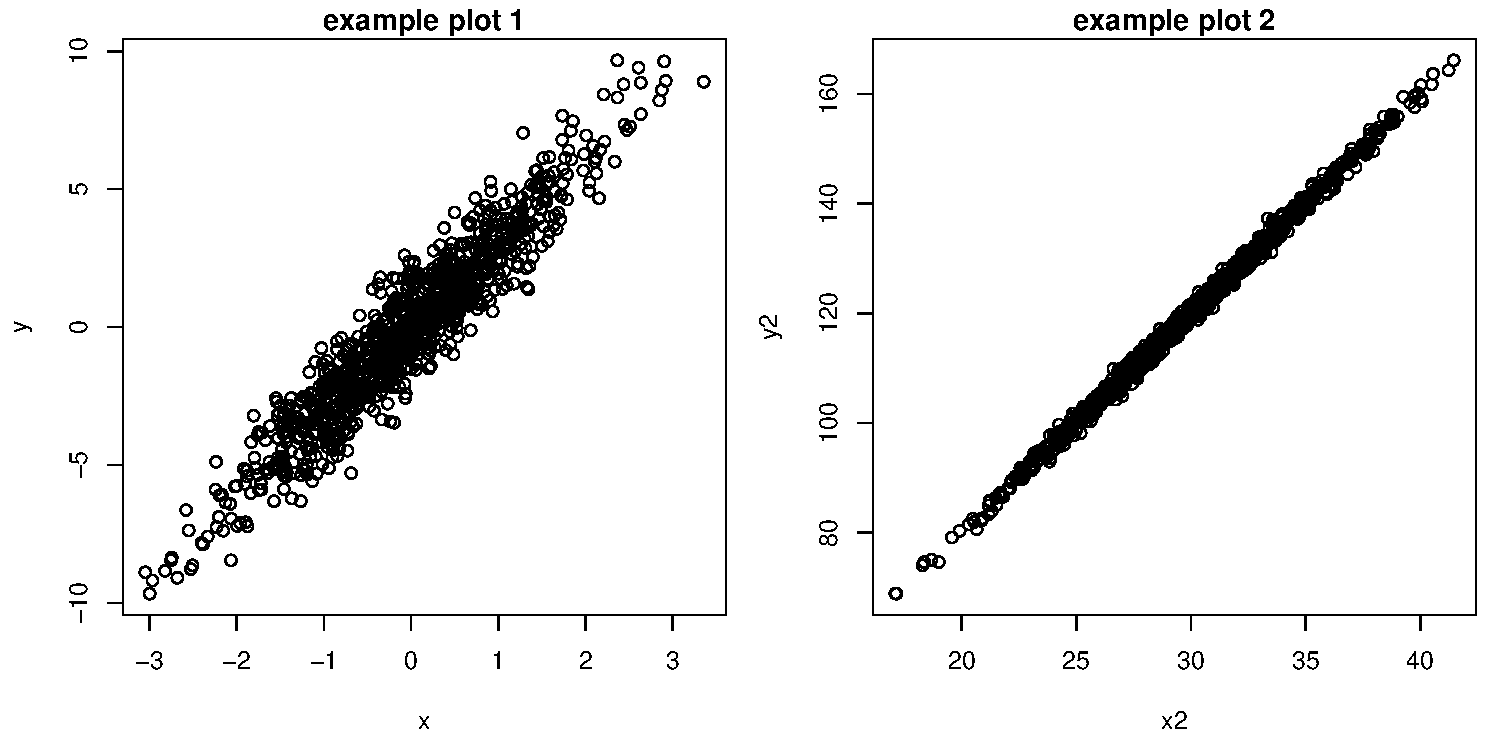
\includegraphics[width=\textwidth]{example_plot.pdf}
\caption{This is an example plot that is just for practice because I don't know how to use GitHub with RStudio very well. Once I figure out all of the weird syntax and point-and-click crap in RStudio, I am game!!!}
\end{tcolorbox}
\end{figure}
%\end{tcolorbox}


\end{document}
